% Options for packages loaded elsewhere
\PassOptionsToPackage{unicode}{hyperref}
\PassOptionsToPackage{hyphens}{url}
\PassOptionsToPackage{dvipsnames,svgnames,x11names}{xcolor}
%
\documentclass[
  letterpaper,
  DIV=11,
  numbers=noendperiod]{scrreprt}

\usepackage{amsmath,amssymb}
\usepackage{iftex}
\ifPDFTeX
  \usepackage[T1]{fontenc}
  \usepackage[utf8]{inputenc}
  \usepackage{textcomp} % provide euro and other symbols
\else % if luatex or xetex
  \usepackage{unicode-math}
  \defaultfontfeatures{Scale=MatchLowercase}
  \defaultfontfeatures[\rmfamily]{Ligatures=TeX,Scale=1}
\fi
\usepackage{lmodern}
\ifPDFTeX\else  
    % xetex/luatex font selection
\fi
% Use upquote if available, for straight quotes in verbatim environments
\IfFileExists{upquote.sty}{\usepackage{upquote}}{}
\IfFileExists{microtype.sty}{% use microtype if available
  \usepackage[]{microtype}
  \UseMicrotypeSet[protrusion]{basicmath} % disable protrusion for tt fonts
}{}
\makeatletter
\@ifundefined{KOMAClassName}{% if non-KOMA class
  \IfFileExists{parskip.sty}{%
    \usepackage{parskip}
  }{% else
    \setlength{\parindent}{0pt}
    \setlength{\parskip}{6pt plus 2pt minus 1pt}}
}{% if KOMA class
  \KOMAoptions{parskip=half}}
\makeatother
\usepackage{xcolor}
\setlength{\emergencystretch}{3em} % prevent overfull lines
\setcounter{secnumdepth}{5}
% Make \paragraph and \subparagraph free-standing
\ifx\paragraph\undefined\else
  \let\oldparagraph\paragraph
  \renewcommand{\paragraph}[1]{\oldparagraph{#1}\mbox{}}
\fi
\ifx\subparagraph\undefined\else
  \let\oldsubparagraph\subparagraph
  \renewcommand{\subparagraph}[1]{\oldsubparagraph{#1}\mbox{}}
\fi


\providecommand{\tightlist}{%
  \setlength{\itemsep}{0pt}\setlength{\parskip}{0pt}}\usepackage{longtable,booktabs,array}
\usepackage{calc} % for calculating minipage widths
% Correct order of tables after \paragraph or \subparagraph
\usepackage{etoolbox}
\makeatletter
\patchcmd\longtable{\par}{\if@noskipsec\mbox{}\fi\par}{}{}
\makeatother
% Allow footnotes in longtable head/foot
\IfFileExists{footnotehyper.sty}{\usepackage{footnotehyper}}{\usepackage{footnote}}
\makesavenoteenv{longtable}
\usepackage{graphicx}
\makeatletter
\def\maxwidth{\ifdim\Gin@nat@width>\linewidth\linewidth\else\Gin@nat@width\fi}
\def\maxheight{\ifdim\Gin@nat@height>\textheight\textheight\else\Gin@nat@height\fi}
\makeatother
% Scale images if necessary, so that they will not overflow the page
% margins by default, and it is still possible to overwrite the defaults
% using explicit options in \includegraphics[width, height, ...]{}
\setkeys{Gin}{width=\maxwidth,height=\maxheight,keepaspectratio}
% Set default figure placement to htbp
\makeatletter
\def\fps@figure{htbp}
\makeatother
\newlength{\cslhangindent}
\setlength{\cslhangindent}{1.5em}
\newlength{\csllabelwidth}
\setlength{\csllabelwidth}{3em}
\newlength{\cslentryspacingunit} % times entry-spacing
\setlength{\cslentryspacingunit}{\parskip}
\newenvironment{CSLReferences}[2] % #1 hanging-ident, #2 entry spacing
 {% don't indent paragraphs
  \setlength{\parindent}{0pt}
  % turn on hanging indent if param 1 is 1
  \ifodd #1
  \let\oldpar\par
  \def\par{\hangindent=\cslhangindent\oldpar}
  \fi
  % set entry spacing
  \setlength{\parskip}{#2\cslentryspacingunit}
 }%
 {}
\usepackage{calc}
\newcommand{\CSLBlock}[1]{#1\hfill\break}
\newcommand{\CSLLeftMargin}[1]{\parbox[t]{\csllabelwidth}{#1}}
\newcommand{\CSLRightInline}[1]{\parbox[t]{\linewidth - \csllabelwidth}{#1}\break}
\newcommand{\CSLIndent}[1]{\hspace{\cslhangindent}#1}

\KOMAoption{captions}{tableheading}
\makeatletter
\@ifpackageloaded{tcolorbox}{}{\usepackage[skins,breakable]{tcolorbox}}
\@ifpackageloaded{fontawesome5}{}{\usepackage{fontawesome5}}
\definecolor{quarto-callout-color}{HTML}{909090}
\definecolor{quarto-callout-note-color}{HTML}{0758E5}
\definecolor{quarto-callout-important-color}{HTML}{CC1914}
\definecolor{quarto-callout-warning-color}{HTML}{EB9113}
\definecolor{quarto-callout-tip-color}{HTML}{00A047}
\definecolor{quarto-callout-caution-color}{HTML}{FC5300}
\definecolor{quarto-callout-color-frame}{HTML}{acacac}
\definecolor{quarto-callout-note-color-frame}{HTML}{4582ec}
\definecolor{quarto-callout-important-color-frame}{HTML}{d9534f}
\definecolor{quarto-callout-warning-color-frame}{HTML}{f0ad4e}
\definecolor{quarto-callout-tip-color-frame}{HTML}{02b875}
\definecolor{quarto-callout-caution-color-frame}{HTML}{fd7e14}
\makeatother
\makeatletter
\makeatother
\makeatletter
\@ifpackageloaded{bookmark}{}{\usepackage{bookmark}}
\makeatother
\makeatletter
\@ifpackageloaded{caption}{}{\usepackage{caption}}
\AtBeginDocument{%
\ifdefined\contentsname
  \renewcommand*\contentsname{Table of contents}
\else
  \newcommand\contentsname{Table of contents}
\fi
\ifdefined\listfigurename
  \renewcommand*\listfigurename{List of Figures}
\else
  \newcommand\listfigurename{List of Figures}
\fi
\ifdefined\listtablename
  \renewcommand*\listtablename{List of Tables}
\else
  \newcommand\listtablename{List of Tables}
\fi
\ifdefined\figurename
  \renewcommand*\figurename{Figure}
\else
  \newcommand\figurename{Figure}
\fi
\ifdefined\tablename
  \renewcommand*\tablename{Table}
\else
  \newcommand\tablename{Table}
\fi
}
\@ifpackageloaded{float}{}{\usepackage{float}}
\floatstyle{ruled}
\@ifundefined{c@chapter}{\newfloat{codelisting}{h}{lop}}{\newfloat{codelisting}{h}{lop}[chapter]}
\floatname{codelisting}{Listing}
\newcommand*\listoflistings{\listof{codelisting}{List of Listings}}
\makeatother
\makeatletter
\@ifpackageloaded{caption}{}{\usepackage{caption}}
\@ifpackageloaded{subcaption}{}{\usepackage{subcaption}}
\makeatother
\makeatletter
\@ifpackageloaded{tcolorbox}{}{\usepackage[skins,breakable]{tcolorbox}}
\makeatother
\makeatletter
\@ifundefined{shadecolor}{\definecolor{shadecolor}{rgb}{.97, .97, .97}}
\makeatother
\makeatletter
\makeatother
\makeatletter
\makeatother
\ifLuaTeX
  \usepackage{selnolig}  % disable illegal ligatures
\fi
\IfFileExists{bookmark.sty}{\usepackage{bookmark}}{\usepackage{hyperref}}
\IfFileExists{xurl.sty}{\usepackage{xurl}}{} % add URL line breaks if available
\urlstyle{same} % disable monospaced font for URLs
\hypersetup{
  pdftitle={Pediatrics Notes},
  pdfauthor={Department of Child Health   School of Medical Sciences   KNUST},
  colorlinks=true,
  linkcolor={blue},
  filecolor={Maroon},
  citecolor={Blue},
  urlcolor={Blue},
  pdfcreator={LaTeX via pandoc}}

\title{Pediatrics Notes}
\author{Department of Child Health School of Medical Sciences KNUST}
\date{2024-03-06}

\begin{document}
\maketitle
\ifdefined\Shaded\renewenvironment{Shaded}{\begin{tcolorbox}[breakable, interior hidden, frame hidden, borderline west={3pt}{0pt}{shadecolor}, boxrule=0pt, enhanced, sharp corners]}{\end{tcolorbox}}\fi

\renewcommand*\contentsname{Table of contents}
{
\hypersetup{linkcolor=}
\setcounter{tocdepth}{2}
\tableofcontents
}
\bookmarksetup{startatroot}

\hypertarget{preface}{%
\chapter*{Preface}\label{preface}}
\addcontentsline{toc}{chapter}{Preface}

\markboth{Preface}{Preface}

This clinical note was put together by the Professors, Senior Lecturers
and Lecturers in the Department of Child Health, School of Medical
Sciences, Kwame Nkrumah University of Science and Technology. Members of
the Child Health Department include:

Prof Sampson Antwi\\
Prof Daniel Ansong\\
Prof Alex Osei-Akoto\\
Prof Emmanuel O. A. Addo-Yobo\\
Prof Joslin Alexei Dogbe\\
Prof (Mrs) Gyikua Plange-Rhule\\
Dr Samuel Blay Nguah\\
Dr Emmanuel Ameyaw\\
Dr Anthony Enimil\\
Dr (Mrs) Vivian Paintsil\\
Dr Serwaa Asafo-Agyei\\
Dr Charles Hammond\\
Dr (Mrs) Sandra Kwarteng Owusu\\
Dr Adwoa Pokua Boakye Yiadom\\
Dr Naana Ayiwa Wireko Brobby\\
Dr (Mrs) Akua Afriyie Ocran

\part{{History \& Examination}}

\hypertarget{child-history-and-examinaion}{%
\chapter{Child History and
Examinaion}\label{child-history-and-examinaion}}

\hypertarget{neonatal-history-examination}{%
\chapter{Neonatal History \&
Examination}\label{neonatal-history-examination}}

\bookmarksetup{startatroot}

\hypertarget{growth-and-development}{%
\chapter{Growth and Development}\label{growth-and-development}}

\bookmarksetup{startatroot}

\hypertarget{pediatric-anthropometry}{%
\chapter{Pediatric Anthropometry}\label{pediatric-anthropometry}}

\part{{Neonatology}}

\hypertarget{newborn-delivery-and-resusctation}{%
\chapter{Newborn Delivery and
Resusctation}\label{newborn-delivery-and-resusctation}}

\hypertarget{preterm-and-low-birth-weight}{%
\chapter{Preterm and Low Birth
Weight}\label{preterm-and-low-birth-weight}}

\hypertarget{neonatal-jaundice}{%
\chapter{Neonatal Jaundice}\label{neonatal-jaundice}}

\hypertarget{introduction}{%
\section{Introduction}\label{introduction}}

Jaundice is the yellowish discoloration of the skin, eyes and mucous
membranes, caused by a pigment called bilirubin in the blood. Out of 10
term and 10 preterm infants, 6 and 8 of them will develop jaundice
respectively, all in the 1st couple of weeks of life. Universally
accepted as one of the commonest causes of admission and readmission in
the first month of life. At KATH MBU, monthly admissions average between
300 and 400 and about 15 -- 25\% of all these admissions are cases of
neonatal jaundice. Whereas the developed world describes kernicterus as
a rare condition, unfortunately, the same cannot be said for us in
developing countries. On average, cases of severe NNJ have ranged from
2.2\% -- 30.8\% of all jaundice cases, with the monthly mortality from
NNJ ranging from 2.8\% - 15.2\%. Remember, kernicterus is the only
preventable cause of cerebral palsy!

\hypertarget{bilirubin-metabolism}{%
\section{Bilirubin metabolism}\label{bilirubin-metabolism}}

Humans continuously form bilirubin and the liver is the main organ
responsible for the metabolism of bilirubin. For every gram of
Hemoglobin, 35mg of bilirubin is produced.\\
The bilirubin is conjugated by the UGT enzyme, making it water-soluble,
which is then released into the bile before being excreted in the stool
(and urine). It can also be broken down in the intestine by bacterial
enzymes like E. coli. However, at birth, the newborn has several
challenges. The liver is immature, and the levels of UGT are low.
Newborns have β-glucuronidase in the intestinal mucosa/brush border,
which deconjugates the conjugated bilirubin found in the meconium. The
unconjugated bilirubin can now be reabsorbed through the intestinal wall
and recycled back into the circulation. This process is known as the
``enterohepatic circulation of bilirubin''. The gut is sterile and,
subsequently, infants have far fewer bacteria in the gut, and so very
little, if any, bilirubin is reduced to urobilin and stercobilin.

Specifically to newborns more bilirubin is produced, on account of the
short life span of Red Blood Cells and high Hemoglobin levels. The liver
is immature. They also have fewer bacteria and low intestinal enzymatic
activity in the intestine

\hypertarget{types-of-bilirubin}{%
\section{Types of bilirubin}\label{types-of-bilirubin}}

There are two types:

\hypertarget{conjugated-direct-bilirubin}{%
\subsection{Conjugated (Direct)
Bilirubin}\label{conjugated-direct-bilirubin}}

This is water soluble, excreted in the urine and stool, and not toxic to
the brain. However, high amounts could indicate underlying liver disease
or injury.

\hypertarget{unconjugated-indirect-bilirubin}{%
\subsection{Unconjugated (Indirect)
Bilirubin}\label{unconjugated-indirect-bilirubin}}

This is lipid soluble, can cross the blood-brain barrier and is toxic in
high amounts to the brain.

In very high concentrations, unconjugated bilirubin, which is lipid
soluble, is toxic to the developing brain. Once it crosses the
blood-brain barrier and binds to brain tissue and deposits in the
developing brain. Since this is an irreversible process, it leads to
long-term neurological issues and even death.

\hypertarget{types-of-jaundice}{%
\section{Types of Jaundice}\label{types-of-jaundice}}

There are two main types of jaundice:\\

\begin{enumerate}
\def\labelenumi{\arabic{enumi}.}
\tightlist
\item
  Physiological jaundice and
\item
  Pathological jaundice.
\end{enumerate}

There are three main mechanisms for jaundice:\\

\begin{enumerate}
\def\labelenumi{\arabic{enumi}.}
\tightlist
\item
  Increased bilirubin production
\item
  Decreased bilirubin clearance and
\item
  Increased enterohepatic circulation.
\end{enumerate}

\hypertarget{physiological-jaundice}{%
\subsection{Physiological jaundice}\label{physiological-jaundice}}

\hypertarget{increased-bilirubin-production}{%
\subsubsection{Increased bilirubin
production}\label{increased-bilirubin-production}}

in term newborn infants, bilirubin production is 2 -- 3x higher than in
adults. This occurs because newborns have more RBCs and fetal RBCs have
a shorter life span than those in adults. Unfortunately, the liver being
immature, cannot conjugate and excrete all the bilirubin from the
breakdown of all the excess RBCs, thereby resulting in spillover of
bilirubin into the blood.

\hypertarget{bilirubin-clearance-or-excretion}{%
\subsubsection{Bilirubin clearance or
excretion}\label{bilirubin-clearance-or-excretion}}

This is decreased in newborns, mainly due to the low levels of the UGT
enzyme in the liver. UGT activity in term infants at day 7 of age is
approximately 1\% of that of the adult liver and does not reach adult
levels until about 14 weeks of age.

\hypertarget{enterohepatic-circulation}{%
\subsubsection{Enterohepatic
circulation}\label{enterohepatic-circulation}}

The presence of the ß-glucuronidase results in an increase in the
enterohepatic circulation of bilirubin, further increasing the bilirubin
load in the infant. This is a diagnosis of exclusion

\hypertarget{pathological-jaundice}{%
\subsection{Pathological jaundice}\label{pathological-jaundice}}

\hypertarget{definition}{%
\subsubsection{Definition}\label{definition}}

Neonatal jaundice is said to be pathologic if:

\begin{itemize}
\tightlist
\item
  Jaundice in the 1st 24 - 48 hours of life.
\item
  Rate of SB rise \textgreater{} 0.5 mg/dL (8.5µmol/L) per hour
\item
  Jaundice all over the body (including palms \& soles)
\item
  Presence of a danger sign
\item
  History of previous siblings having had jaundice at birth
\item
  Jaundice in a term newborn after 2 weeks of age or in a preterm infant
  after 3 weeks of age
\item
  Direct (conjugated) bilirubin concentration \textgreater{} 20\% of the
  total
\end{itemize}

It can be caused by certain pathologic conditions or exaggeration of the
mechanisms responsible for physiologic neonatal jaundice. Identification
of what is causing the jaundice is useful in guiding management,
including counselling of the parents and what to expect for the next
pregnancy. Most common cause is increased bilirubin production due to
haemolytic disease processes that include the following:

\begin{itemize}
\tightlist
\item
  Isoimmune-mediated haemolysis (e.g., ABO or Rhesus D incompatibility)
\item
  Erythrocyte enzymatic defects, e.g.~G6PD deficiency
\item
  Sepsis, especially Urinary Tract Infection
\item
  Polycythaemia
\item
  Birth Injuries resulting in sequestration of blood within a closed
  space, e.g.~cephalohematoma, subgaleal bleed.
\end{itemize}

\hypertarget{abo-incompatibility}{%
\subsubsection{ABO incompatibility}\label{abo-incompatibility}}

This is one of the most common causes of isoimmune hemolytic disease
during the neonatal period. Infants with blood group A or B, carried by
blood group O mother, will have a positive antibody because of maternal
anti-A or anti-B transfer into the fetal circulation.

\hypertarget{rhesus-incompatibility}{%
\subsubsection{Rhesus Incompatibility}\label{rhesus-incompatibility}}

Rh incompatibility can occur when an Rh-negative pregnant mother is
exposed to Rh-positive fetal red blood cells secondary to feto-maternal
haemorrhage during pregnancy/delivery. As a result, the mother's blood
gets exposed to the fetal circulation and sensitization occurs leading
to maternal antibody production against the foreign Rh antigen. Once
produced, maternal Rh (IgG) antibodies may cross freely from the
placenta to the fetal circulation, where they form antigen-antibody
complexes with Rh- positive fetal RBCs and eventually are destroyed,
resulting in a fetal alloimmune-induced hemolytic anaemia and jaundice.
The first pregnancy is usually not affected, but more antibodies are
produced with each pregnancy making the jaundice worse with each
pregnancy.

\hypertarget{decreased-clearance}{%
\subsubsection{Decreased clearance}\label{decreased-clearance}}

Inherited defects in the gene that encodes the UGT liver enzyme (eg,
Gilbert Syndrome), decrease bilirubin conjugation (eg Crigglar Najjar).
In physiological jaundice, the levels are naturally low, but here, in
addition to the low levels the UGT enzyme is either defective, absent or
has a reduced function. This reduces hepatic bilirubin metabolism and
its clearance thereby increasing the total serum unconjugated bilirubin
levels.

\hypertarget{increased-enterohepatic-circulation}{%
\subsubsection{Increased enterohepatic
circulation}\label{increased-enterohepatic-circulation}}

The major causes are\\

\begin{itemize}
\tightlist
\item
  Breastfeeding jaundice
\item
  Breast milk jaundice
\item
  Impaired intestinal motility is caused by functional or anatomic
  obstruction.
\item
  Congenital hypothyroidism also causes increased enterohepatic
  circulation on account of reduced gut motility.
\end{itemize}

\hypertarget{assessing-for-neonatal-jaundice}{%
\section{Assessing for Neonatal
Jaundice}\label{assessing-for-neonatal-jaundice}}

\begin{itemize}
\tightlist
\item
  Baby should be assessed in natural daylight
\item
  Look for yellow eyes \& skin, check the white part of the eyes only if
  the baby opens the eyes voluntarily.
\item
  You may blanch the skin on the bridge of the nose or the palms/soles
  of the feet if they turn yellow\ldots{}
\item
  Remember that the yellowing spreads from head to toe\ldots{}
\item
  Do not rely on visual inspection alone to estimate the bilirubin level
  in a baby with jaundice!!! It can be very subjective!!
\end{itemize}

\hypertarget{clinical-features}{%
\section{Clinical features}\label{clinical-features}}

The clinical features of neonatal jaundice may include:

\begin{itemize}
\tightlist
\item
  Baby looks yellow! The yellowness appears cephalocaudal.
\item
  May not be as active as he/she used to be
\item
  Lethargic/hypotonic
\item
  Weak cry, irritable
\item
  Poor feeding
\item
  High-pitched cry / poor cry
\item
  Seizures
\item
  Arching of the neck/back
\end{itemize}

Thus to evaluate a child with jaundice we:

\begin{itemize}
\tightlist
\item
  Determine birth weight, gestation and postnatal age (in hours)
\item
  Assess clinical condition (well or ill)
\item
  Degree of jaundice (visual inspection, SBR etc)
\item
  Look for evidence of kernicterus / BIND
\end{itemize}

\hypertarget{management}{%
\section{Management}\label{management}}

The general principle of treatment includes

\begin{itemize}
\tightlist
\item
  Encourage frequent exclusive breastfeeding.
\item
  Start Intravenous fluids only when there are signs of dehydration
\item
  Watch out for danger signs
\item
  Pathologic Neonatal jaundice is treated with

  \begin{itemize}
  \tightlist
  \item
    Phototherapy
  \item
    Exchange Blood Transfusion (EBT)
  \item
    Antibiotics
  \end{itemize}
\end{itemize}

Be interested in the cause as this will serve as a guide in the
management of the baby and direct your counselling as well as impact on
subsequent pregnancies Loads of information in the maternal and child
health record book, Gravidity and Parity, G6PD status, maternal Blood
group \& Rhesus status etc

\hypertarget{investigations}{%
\subsection{Investigations}\label{investigations}}

This should include but not be restricted to

\begin{itemize}
\tightlist
\item
  Serum Bilirubin (conjugated, unconjugated and total)
\item
  Full Blood Count
\item
  G6PD screening
\item
  Blood Culture \& Sensitivity
\item
  Baby's blood group (only necessary if mother's blood group is O)
\item
  Others include Direct Coomb's test, Urine C \& S etc
\end{itemize}

\hypertarget{phototherapy}{%
\subsection{Phototherapy}\label{phototherapy}}

Phototherapy is the use of visible light to treat high levels of serum
bilirubin in the newborn.

\begin{figure}

{\centering 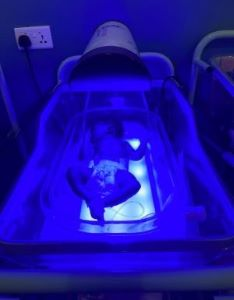
\includegraphics{neo-phototherapy.jpg}

}

\caption{Phototherapy Unit}

\end{figure}

The dose of phototherapy is a key factor in how quickly it works. The
dose in turn is determined by:

\begin{itemize}
\tightlist
\item
  The wavelength of the light
\item
  The intensity of the light (irradiance)
\item
  The distance between the light and the baby
\item
  The body's surface area is exposed to the light.
\end{itemize}

Effective phototherapy lowers serum bilirubin levels by converting the
lipid-soluble bilirubin into water-soluble forms that can easily be
excreted in the stool and urine Phototherapy also prevents the need for
an Exchange Blood Transfusion and prevents bilirubin from depositing in
the brain. The breakdown of bilirubin begins almost instantaneously when
the skin is exposed to light, hence, phototherapy should be started as
early as possible.

In initiating phototherapy, always note the time the baby's SBR sample
is being taken and estimate the age in hours up until that time.
Interpret bilirubin levels according to the baby's postnatal age in
hours and manage the bilirubin levels according to the threshold table
Start phototherapy if the SBR plots on or above the line appropriate for
age (in hours) and gestational age If the SBR plots just underneath the
line, repeat the SBR after 6 hours or start phototherapy if a repeat is
not feasible. Repeat the SBR at least 24 to 48 hours after initiation of
phototherapy. Discontinue phototherapy when the SBR plots below the
line.

The side effects of phototheratpy include:

\begin{itemize}
\tightlist
\item
  Increase insensible water loss
\item
  Loose stools
\item
  Skin rash
\item
  Bronze baby syndrome
\item
  Hypo- or Hyperthermia
\item
  Interruption of mother-baby bonding
\end{itemize}

\hypertarget{sunlight-therapy}{%
\subsection{Sunlight Therapy}\label{sunlight-therapy}}

Works for physiological jaundice, however, one can never tell by looking
at a baby what kind of jaundice a baby has Err on the side of caution,
at least always have the SBR checked first Remember prolonged exposure
to UV rays can be harmful to the developing skin Baby cannot be put in
the light for more than 30 minutes in a day Even most of the available
literature and studies that recommend sunlight still advice that if the
jaundice is severe, the baby must be managed in the hospital!! A serum
bilirubin high enough to warrant treatment should be managed in the
hospital.

\hypertarget{exchange-blood-transfusion}{%
\subsection{Exchange Blood
Transfusion}\label{exchange-blood-transfusion}}

Provides a means of rapid reduction of circulating bilirubin in the
blood. Involves manual removal of the baby's blood and simultaneously
replacing it with compatible donor blood.

\begin{figure}

{\centering 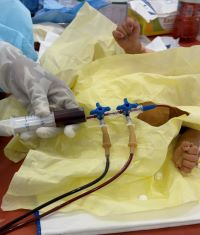
\includegraphics{neo-ebt.jpg}

}

\caption{Exchange Blood Transfusion}

\end{figure}

In addition to reducing bilirubin levels, EBT removes partially
hemolyzed RBCs, RBCs coated with antibodies and circulating
immunoglobulins.

\begin{figure}

{\centering 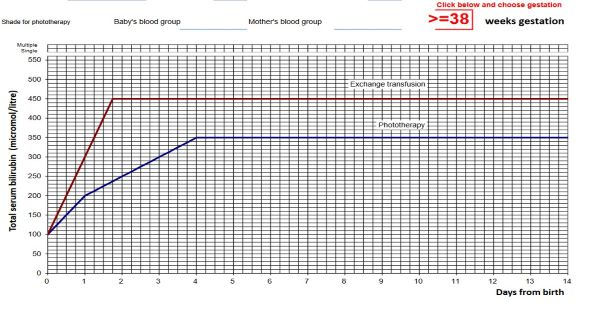
\includegraphics{ebt-chart.jpg}

}

\caption{Bilirubin Graph (\textgreater{} 38 weeks)}

\end{figure}

Complication of exchange blood transfusion include:

\begin{itemize}
\tightlist
\item
  Cardiac \& respiratory disorders
\item
  Shock due to bleeding or inadequate replacement of blood infection
\item
  Catheter-related complications
\item
  Changes in the composition of the blood (high or low potassium, low
  calcium, low glucose, changes in pH)
\item
  Thrombocytopenia
\item
  And the rare but serious complications of air embolism, portal
  hypertension, and necrotizing enterocolitis.
\end{itemize}

\hypertarget{intravenous-immunoglobins}{%
\subsection{Intravenous Immunoglobins}\label{intravenous-immunoglobins}}

Treatment with intravenous immunoglobulin (IVIG) has been suggested as
an alternative therapy to Exchange Blood Transfusion for isoimmune
hemolytic jaundice to reduce the need for Exchange Blood Transfusion and
duration of phototherapy and hospitalization in isoimmune hemolytic
disease of the newborn. It has been proposed that IVIG blocks the
binding of the antibody to the antigen. With this blockade, hemolysis no
longer occurs.

\hypertarget{long-term-complications}{%
\section{Long term complications}\label{long-term-complications}}

The effects of bilirubin toxicity include

\begin{itemize}
\tightlist
\item
  Hearing loss
\item
  Cerebral palsy
\item
  Mental retardation
\item
  Dental complications
\item
  Delayed developmental milestones
\item
  Seizure and visual disorders
\end{itemize}

\hypertarget{recommendations}{%
\section{Recommendations}\label{recommendations}}

\begin{itemize}
\tightlist
\item
  Always err on the side of caution
\item
  An SBR is always more objective
\item
  Look out for danger signs
\item
  As much breastmilk as possible by any means necessary
\item
  Sunlight therapy is not recommended, if the baby is yellow enough for
  you to want to put him/her under the sun, then the baby needs to be
  brought to the hospital!
\end{itemize}

\hypertarget{newborn-feeding}{%
\chapter{Newborn Feeding}\label{newborn-feeding}}

\hypertarget{neonatal-delivery-conditions}{%
\chapter{Neonatal Delivery
Conditions}\label{neonatal-delivery-conditions}}

\hypertarget{the-health-newborn}{%
\section{The health newborn}\label{the-health-newborn}}

\begin{itemize}
\tightlist
\item
  Cries / Breathes normally
\item
  Pink all over
\item
  Well-flexed \& moves all limbs spontaneously
\item
  Suckles well at the breast
\item
  Birth weight 2.5 -- 4.0kg
\item
  Normal vitals signs
\end{itemize}

\hypertarget{occurrences-at-birth}{%
\section{Occurrences at birth}\label{occurrences-at-birth}}

\begin{itemize}
\tightlist
\item
  The fluid in the alveoli is absorbed and replaced by air. If the
  transition is not smooth, it results in insufficient oxygen delivery
  to the vital organs\ldots{}
\item
  Poor muscle tone
\item
  Respiratory distress or depression
\item
  Slow heart rate
\item
  Low BP
\item
  Cyanosis
\end{itemize}

\hypertarget{birth-asphyxia}{%
\section{Birth Asphyxia}\label{birth-asphyxia}}

\hypertarget{definition-1}{%
\subsection{Definition}\label{definition-1}}

\begin{tcolorbox}[enhanced jigsaw, left=2mm, toptitle=1mm, colbacktitle=quarto-callout-important-color!10!white, opacityback=0, bottomtitle=1mm, toprule=.15mm, titlerule=0mm, colback=white, breakable, opacitybacktitle=0.6, title=\textcolor{quarto-callout-important-color}{\faExclamation}\hspace{0.5em}{World Health Organisation definition}, leftrule=.75mm, arc=.35mm, colframe=quarto-callout-important-color-frame, rightrule=.15mm, bottomrule=.15mm, coltitle=black]

Birth Asphyxia is the medical condition resulting from deprivation of
oxygen in the newborn that lasts long enough during the birth process to
cause harm, usually to the brain.

\end{tcolorbox}

\hypertarget{risk-factors}{%
\subsection{Risk factors}\label{risk-factors}}

Any condition that will lead to impairment of oxygenation or blood flow
to the newborn's brain in the perinatal period. These include:

\begin{itemize}
\tightlist
\item
  Prolonged labour (CPD)
\item
  Placental failure
\item
  Cord around the neck
\item
  Problems with oxygenation of maternal blood / maternal disease
\item
  Anaemia and bleeding in the baby
\item
  Congenital heart disease
\item
  Infections
\item
  Deficient medical skills and or knowledge
\end{itemize}

\hypertarget{presentation}{%
\subsection{Presentation}\label{presentation}}

The asphyxiated baby may have any of the following:

\begin{itemize}
\tightlist
\item
  Poor Apgar Scores
\item
  May not cry at birth
\item
  Floppy/spastic
\item
  Breathing problems
\item
  Unresponsive
\item
  Seizures
\item
  Irritable
\end{itemize}

\hypertarget{the-apgar-score}{%
\subsection{The APGAR Score}\label{the-apgar-score}}

It is an objective method of quantifying the newborn's condition. And is
useful for conveying information about the newborn's overall status and
response to resuscitation

\begin{longtable}[]{@{}
  >{\raggedright\arraybackslash}p{(\columnwidth - 6\tabcolsep) * \real{0.1717}}
  >{\raggedright\arraybackslash}p{(\columnwidth - 6\tabcolsep) * \real{0.1414}}
  >{\raggedright\arraybackslash}p{(\columnwidth - 6\tabcolsep) * \real{0.2727}}
  >{\raggedright\arraybackslash}p{(\columnwidth - 6\tabcolsep) * \real{0.4141}}@{}}
\caption{The APGAR Score}\tabularnewline
\toprule\noalign{}
\begin{minipage}[b]{\linewidth}\raggedright
\end{minipage} & \begin{minipage}[b]{\linewidth}\raggedright
0
\end{minipage} & \begin{minipage}[b]{\linewidth}\raggedright
1
\end{minipage} & \begin{minipage}[b]{\linewidth}\raggedright
2
\end{minipage} \\
\midrule\noalign{}
\endfirsthead
\toprule\noalign{}
\begin{minipage}[b]{\linewidth}\raggedright
\end{minipage} & \begin{minipage}[b]{\linewidth}\raggedright
0
\end{minipage} & \begin{minipage}[b]{\linewidth}\raggedright
1
\end{minipage} & \begin{minipage}[b]{\linewidth}\raggedright
2
\end{minipage} \\
\midrule\noalign{}
\endhead
\bottomrule\noalign{}
\endlastfoot
\textbf{Heart Rate} & 0 & \textless100 & \textgreater=100 \\
\textbf{Respiration} & 0 & Weak or Irregular & Good Cry \\
\textbf{Reaction} & None & Slight & Good \\
\textbf{Colour} & Blue or Pale & Pink body limbs blue & All pink \\
\textbf{Tone} & Limp & Some movement & Active movement, limbs well
flexed \\
\end{longtable}

8-10 = No Asphyxia\\
5-7 = Mild Asphyxia\\
3-4 = Moderate Asphyxia\\
0-2 = Severe Asphyxia\\

\hypertarget{management-1}{%
\subsection{Management}\label{management-1}}

\begin{itemize}
\tightlist
\item
  Largely supportive
\item
  Newborn resuscitation/oxygenation
\item
  Correction of fluid \& electrolyte imbalances including shock
\item
  Control of seizures
\item
  Treatment of any underlying infection
\item
  Look out for birth injuries
\item
  Active cooling found to improve neurological outcome
\item
  Temperature maintenance
\item
  Full Blood Count, Culture \& Sensitivity, Blood glucose etc
\item
  Serum electrolytes: Na, K, Ca \& Mg
\item
  Start empiric 1st line antibiotics according to protocol: / X'pen \&
  Gentamycin
\item
  Start IV Fluids at 50ml/kg (Plain 10\% Dextrose).
\item
  Pass a urethral catheter and monitor the baby's urine output.
\item
  The target temperature of the baby is 36.50C -- 37.50C
\end{itemize}

\hypertarget{hypoxemic-ischaemic-encephalopathy}{%
\subsection{Hypoxemic Ischaemic
Encephalopathy}\label{hypoxemic-ischaemic-encephalopathy}}

\begin{itemize}
\tightlist
\item
  The most important consequence of birth asphyxia is
\item
  The outcome ranges from complete recovery to death
\item
  25 - 30\% end up with permanent damage like Cerebral palsy \& Mental
  retardation
\item
  Prognosis dependent on gestational age, management of metabolic \&
  cardiopulmonary complications \& the severity of the encephalopathy
\item
  Subsequent competent care and available facilities also influence the
  outcome
\end{itemize}

This is the first type of humeral fracture

\begin{figure}

{\centering 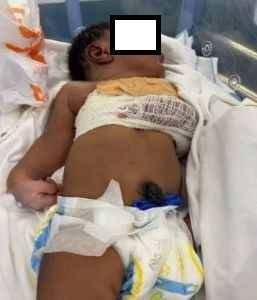
\includegraphics{humeral-fracture-1.jpg}

}

\caption{Humeral Fracture (immobilised)}

\end{figure}

And this is another one

\begin{figure}

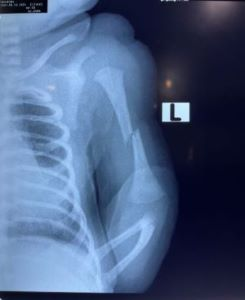
\includegraphics{humeral-fracture-2.jpg} \hfill{}

\caption{X-ray of a humeral fracture}

\end{figure}

\part{{Pulmonology}}

\hypertarget{respiratory-disorders-i}{%
\chapter{Respiratory Disorders I}\label{respiratory-disorders-i}}

\hypertarget{respiratory-disorders-ii}{%
\chapter{Respiratory Disorders II}\label{respiratory-disorders-ii}}

\part{{Cardiology}}

\hypertarget{anatomy-physiology-pathology}{%
\chapter{Anatomy, physiology \&
Pathology}\label{anatomy-physiology-pathology}}

\hypertarget{anatomy-physiology-and-pathology}{%
\section{Anatomy, physiology and
Pathology}\label{anatomy-physiology-and-pathology}}

The heart is located in the mediastinum of the chest, bounded anteriorly
by the sternum, posteriorly by the spine and laterally by the lungs.
Externally, the right ventricle is anterior. Most of the left ventricle,
left atrium and right atrium are posterior. internally the right and
left atria are separated by the tricuspid and mitral valves
respectively. The arterial supply of the heart is through the coronary
arteries while venous drainage is through the coronary sinus. The aorta
and pulmonary arteries arise from the left and right ventricles. The
heart has three layers:

\begin{enumerate}
\def\labelenumi{\arabic{enumi}.}
\tightlist
\item
  Endocardium: Inner epithelial layer of the heart
\item
  Myocardium: Muscular part of the heart
\item
  Pericardium: Outer layers of the heart. Divided into the visceral and
  parietal pericardium.
\end{enumerate}

Venous blood enters the right atrium through the inferior and superior
vena cavae. It empties in atrial systole into the right ventricle
through the tricuspid valve. It then moves on through the pulmonary
valve in ventricular systole, to the pulmonary artery and the the lungs.
Blood returning from the lungs enters the right atrium through the four
pulmonary veins. In atrial systole, it moves onto the left ventricle
through the mitral valve. Finally, it empties into the aorta through the
aortic valve.

The heart has an inherent electrical system that automatically
depolarises it. The parts are:

\begin{enumerate}
\def\labelenumi{\arabic{enumi}.}
\tightlist
\item
  The SinoAtrial (SA) node: This is the pacemaker of the heart and
  depolarises the two atria.
\item
  AtrioVentricular (AV) node: Receives impulses from the SA node, delays
  a bit before propagating it further
\item
  His-purkinje fibre system. Responsible for the spread of electrical
  impulses to the ventricles
\end{enumerate}

\textbf{Heart as a pump}\\
There is a difference in the pumping action of the heart in utero and
after birth.

\begin{enumerate}
\def\labelenumi{\arabic{enumi}.}
\tightlist
\item
  Fetal

  \begin{itemize}
  \tightlist
  \item
    Most work is done by the Right ventricle
  \item
    The right Ventricle is therefore relatively hypertrophic
  \item
    Only 15\% of the cardiac output is pumped into the lungs
  \end{itemize}
\item
  After birth

  \begin{itemize}
  \tightlist
  \item
    Gradual transition to Left ventricle dominance
  \item
    Gradual fall in pulmonary pressure (over 6 weeks)
  \item
    The left ventricle does most of the work and becomes thicker than
    the right
  \end{itemize}
\end{enumerate}

\textbf{Systolic and diastolic functions}

\emph{Systole}: This is the contractile phase of the heart. It starts
with the atrium so it empties into the ventricles before the ventricle's
subsequent contract.

\emph{Diastole}: This is the relaxation phase where the heart relaxes
and lets in blood. It also starts with the atrium and then the
ventricles.

\emph{Compliance}: This describes how easily the heart chamber relaxes
in response to the inflow of blood.

\textbf{Cardiac Pressures}

The pressures in the heart vary for different ages and individuals.
Generally, the pressure in the atria are lower than that in the
ventricles. Also, the pea systolic pressure in the left ventricle is
higher than in the right. The diastolic pressure in the left ventricle
is however lower than the right ventricle. In the typical adult heart,
the following pressures are often observed. Also, both systolic and
diastolic pressure in the aorta is higher than that in the pulmonary
artery.

Systolic pressure in general is generated by the ventricles. In
conditions such as coarctation of the aorta, aortic stenosis and
pulmonary hypertension, the ventricles end up increasing their workload
to generate enough pressure. The diastolic pressure on the other hand is
maintained by the closure of the aortic and pulmonary valves. Thus
incompetent pulmonary or aortic valve leads to a decrease in diastolic
pressure in the the tow vessels respectively.

\hypertarget{evaluating-heart-diseases}{%
\chapter{Evaluating Heart Diseases}\label{evaluating-heart-diseases}}

\hypertarget{heart-failure}{%
\chapter{Heart Failure}\label{heart-failure}}

\hypertarget{atrial-septal-defect}{%
\chapter{Atrial Septal Defect}\label{atrial-septal-defect}}

\hypertarget{section}{%
\section{}\label{section}}

\hypertarget{introducion}{%
\section{Introducion}\label{introducion}}

\begin{enumerate}
\def\labelenumi{\arabic{enumi}.}
\tightlist
\item
  Defect in the inter-atrial septum
\item
  5-10\% of all CHD
\item
  Types

  \begin{itemize}
  \tightlist
  \item
    Secundum ASD (most common, 50-70\%)
  \item
    Primum ASD (30\%)
  \item
    Sinus venosus ASD
  \item
    Coronary sinus ASD
  \end{itemize}
\end{enumerate}

\hypertarget{pathophysiology}{%
\section{Pathophysiology}\label{pathophysiology}}

\begin{itemize}
\tightlist
\item
  Left to right shunting and thus acyanotic
\item
  leads to volume overload of the right atrium, ventricle, pulmonary
  artery and pulmonary oedema
\item
  Consequent dilatation of the right atrium and ventricles
\item
  Minimal pressure transmitted so no significant pressure overload
\item
  Consequently, pulmonary oedema is usually insignificant
\item
  Rarely have overt heart failure
\item
  However, long-standing liaison or a very big lesion with a
  pulmonary-to-systemic flow ratio of 2 or more will lead to heart
  failure and pulmonary hypertension after about 15 to 20 years No
  Reversal of shunt
\end{itemize}

\hypertarget{clinical-presentatoin}{%
\section{Clinical presentatoin}\label{clinical-presentatoin}}

\begin{itemize}
\tightlist
\item
  Usually asymptomatic except for big lesion with high Qp: Qs
\item
  They often have slender bodies
\item
  Auscultation reveals a widely fixed split-second heart sound and a
  grade 2/6 to 3/6 ejection systolic murmur at the upper sternal border
\item
  Many are almost silent, especially the small lesions which are often
  detected during an echocardiogram for another reason
\end{itemize}

\hypertarget{investigations-1}{%
\section{Investigations}\label{investigations-1}}

\begin{itemize}
\tightlist
\item
  Bedside SpO2 is usually normal and hence an acyanotic heart disease
\item
  In older patients, a chest x-ray may show

  \begin{itemize}
  \tightlist
  \item
    Cardiomegaly
  \item
    Prominent pulmonary artery
  \item
    Increased vascular markings
  \end{itemize}
\item
  The electrocardiogram may show

  \begin{itemize}
  \tightlist
  \item
    Right axis deviation due to the right ventricular dilatation
  \item
    Right atrial enlargement
  \end{itemize}
\item
  An echocardiogram is diagnostic as it visualises the defect, and
  quantifies the shunt and other chamber sizes.
\item
  Cardiac catheterization is often done in long-standing cases to detect
  complications that may have arisen.
\end{itemize}

\hypertarget{natural-history}{%
\section{Natural history}\label{natural-history}}

\begin{itemize}
\tightlist
\item
  Most ASDs will close spontaneously by 4 years, with smaller ones
  having a higher closure rate than bigger ones. A long-standing large
  defect however leads to chronic heart failure and pulmonary
  hypertension in early adulthood.
\item
  Arrhythmias may arise because of the dilated right atrium.
\item
  Though there are reported cases of paradoxical strokes in patients
  with ASDs, it remains an uncommon occurrence.
\item
  Infective endocarditis is also rare in ASDs.
\end{itemize}

\hypertarget{treatment}{%
\section{Treatment}\label{treatment}}

There is no need for exercise restriction or prophylaxis for
endocarditis. If there is no sign of heart failure, a device closure is
often done after infancy or a surgical closure at 2-4 years of age.
However, if there is heart failure, Medical treatment for heart failure
is immediately instituted. Then a planned device closure or surgical
closure can be done within the first year of life.

\hypertarget{prognosis}{%
\section{Prognosis}\label{prognosis}}

Prognosis is generally good with many living into adulthood even without
corrective surgery. Post-surgical mortality i currently less the 0.5\%.
The patient will need very little long-term follow-up after the
corrective surgery.

\hypertarget{ventricular-septal-defect}{%
\chapter{Ventricular Septal Defect}\label{ventricular-septal-defect}}

\hypertarget{patent-ductus-arteriosus}{%
\chapter{Patent Ductus Arteriosus}\label{patent-ductus-arteriosus}}

\hypertarget{coarctation-of-the-aorta}{%
\chapter{Coarctation of the Aorta}\label{coarctation-of-the-aorta}}

\hypertarget{tetralogy-of-fallot}{%
\chapter{Tetralogy of Fallot}\label{tetralogy-of-fallot}}

\hypertarget{rheumatic-heart-disease}{%
\chapter{Rheumatic Heart Disease}\label{rheumatic-heart-disease}}

\hypertarget{infective-endocarditis}{%
\chapter{Infective Endocarditis}\label{infective-endocarditis}}

\hypertarget{endomyocardial-fibrosis}{%
\chapter{Endomyocardial Fibrosis}\label{endomyocardial-fibrosis}}

\hypertarget{miscellaneous-conditions}{%
\chapter{Miscellaneous Conditions}\label{miscellaneous-conditions}}

\part{{Infectious Diseases}}

\hypertarget{immunodeficiencies}{%
\chapter{Immunodeficiencies}\label{immunodeficiencies}}

\hypertarget{hiv}{%
\chapter{HIV}\label{hiv}}

\hypertarget{bacterial-sepsis-uti}{%
\chapter{Bacterial Sepsis \& UTI}\label{bacterial-sepsis-uti}}

\hypertarget{tuberculosis}{%
\chapter{Tuberculosis}\label{tuberculosis}}

\hypertarget{immunization}{%
\chapter{Immunization}\label{immunization}}

\hypertarget{viral-infections}{%
\chapter{Viral Infections}\label{viral-infections}}

\part{{Oncology}}

\hypertarget{pediatric-oncology-i}{%
\chapter{Pediatric Oncology I}\label{pediatric-oncology-i}}

\hypertarget{pediatric-oncology-ii}{%
\chapter{Pediatric Oncology II}\label{pediatric-oncology-ii}}

\part{{Nephrology}}

\hypertarget{hypertension}{%
\chapter{Hypertension}\label{hypertension}}

\hypertarget{the-concept-of-blood-pressure}{%
\section{The Concept of Blood
Pressure}\label{the-concept-of-blood-pressure}}

Blood pressure is the force exerted by the blood against any unit area
of the vessel wall. Physiologically,
\[BP = CO \times TPR = SV \times HR \times TPR\] Where:

\begin{itemize}
\tightlist
\item
  \(HR\) is the Heart Rate
\item
  \(BP\) is the Blood Pressure
\item
  \(TPR\) is the Total Peripheral Resistance
\item
  \(CO\) is the Cardiac Output
\item
  \(SV\) is the stroke volume
\end{itemize}

\hypertarget{ways-of-measuring-blood-pressure}{%
\section{Ways of measuring blood
pressure}\label{ways-of-measuring-blood-pressure}}

\begin{enumerate}
\def\labelenumi{\arabic{enumi}.}
\tightlist
\item
  \textbf{Direct intra-arterial} measurements by placing a catheter into
  the vessel and measuring the pressure ``in line'' with the vessel
  (end-on-pressure). This method is used by physiologists and
  Intensivists. The principle is employed in the measurements of central
  venous pressure and intracranial pressure in clinical practice.
\item
  \textbf{The auscultatory method} is done with the use of a
  sphygmomanometer (either mercury or aneroid) and a stethoscope. This
  is the gold standard in clinical practice. Korotkoff sounds 1 and 5
  sounds are measured for systolic and diastolic bleed pressures
  respectively. Values obtained are generally lower than direct \&
  oscillometric measurements.
\item
  \textbf{The palpation method} (flush technique) is performed with the
  use of a sphygmomanometer and palpating finger. Largely unreliable.
  Only systolic blood pressure can be measured with this technique. The
  palpated pulse is generally lower than Korotkoff sound 1 by 10mmHg.
\item
  \textbf{The oscillometric method} uses a sphygmomanometer and a
  monitor e.g.~digital blood pressure devices and Dynamap. Here,
  pulsatile blood flow through arterial wall oscillations is transmitted
  to the cuff encircling the extremity. Korotkoff sound 1 is recorded at
  the point of rapid increase in oscillation amplitude. Korotkoff sound
  5 is recorded as the point of a sudden decrease in oscillation
  amplitude. Values obtained by oscillometric measurements are generally
  higher than auscultatory.
\item
  \textbf{Doppler ultrasound technique}: Here a Doppler ultrasound is
  held over the pulse to magnify the sound so that it is audible without
  a stethoscope. The sound detected may be 5mmHg higher than Korotkoff
  sound 1.
\item
  \textbf{Ambulatory blood pressure measurements}. Here, multiple
  measurements are recorded over time (e.g.~24 hours) with digital
  devices attached to the limb whilst the patient engages in normal
  activities outside the hospital. Results are analysed on a computer or
  paper tracer built into the device using the mean of the readings. It
  provides a truer picture of blood pressure trends useful in diagnosing
  ``white coat hypertension'' and nocturnal hypertension (absence of a
  normal physiological drop in blood pressure during sleep).
\end{enumerate}

\hypertarget{definition-of-hypertension-in-children}{%
\section{Definition of Hypertension in
children}\label{definition-of-hypertension-in-children}}

\textbf{In adults}, the epidemiological definition is based on the risk
of adverse events (e.g.~Stroke) being\textgreater140/90mmHg. \textbf{In
children}, hypertension is defined statistically based on normative
data: ≥ 95th centile for age, height, and gender (Refer to height
centile chart and blood pressure levels). By this statistical
definition, 5\% of children will be classified as hypertensives. Other
definitions include:

\begin{itemize}
\item
  \textbf{Normal blood pressure}: \textless{} 90th centile for age,
  height, and sex.
\item
  \textbf{Pre-Hypertension}: 90th -- \textless95th centile for age,
  height, and sex
\item
  \textbf{Stage 1 Hypertension}: 95th - 99th + 5 mmHg
\item
  \textbf{Stage 2 Hypertension}: \emph{\textgreater{} 99th centile +
  5mmHg}

  A sample of the blood pressure chart is shown below.
\end{itemize}

\begin{figure}

{\centering 

\href{https://www.bing.com/ck/a?!\&\&p=03173e8901eee155JmltdHM9MTcwODkwNTYwMCZpZ3VpZD0xMTM3ZDFjZC1mMmJmLTY1YzctMjQ4My1jMmI3ZjNkODY0NjUmaW5zaWQ9NTE5NA\&ptn=3\&ver=2\&hsh=3\&fclid=1137d1cd-f2bf-65c7-2483-c2b7f3d86465\&psq=blood+pressure+pediatric+centile+charts+pdf\&u=a1aHR0cHM6Ly93d3cubmhsYmkubmloLmdvdi9maWxlcy9kb2NzL2d1aWRlbGluZXMvY2hpbGRfdGJsLnBkZg\&ntb=1}{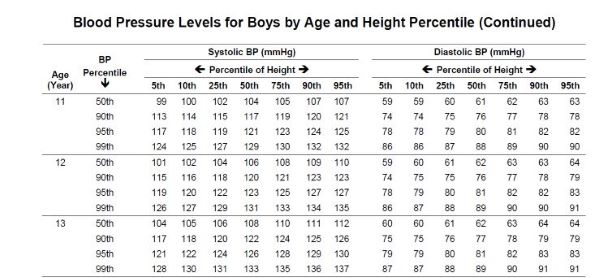
\includegraphics{bpchart.jpg}}

}

\caption{Blood Pressure Centile Chart}

\end{figure}

\hypertarget{plotting-the-blood-pressure-centile}{%
\section{Plotting the blood pressure
centile}\label{plotting-the-blood-pressure-centile}}

\begin{enumerate}
\def\labelenumi{\arabic{enumi}.}
\tightlist
\item
  Measure the child's height
\item
  Determine the height centile. If the height centile falls between 2
  centiles, use the closest centile. Otherwise, use the lower height
  centile.
\item
  Determine the blood pressure centile.
\item
  Classify blood pressure using the definitions above.
\end{enumerate}

\hypertarget{hypertensive-emergency}{%
\section{Hypertensive emergency}\label{hypertensive-emergency}}

This is an acutely elevated blood pressure with evidence of threatening
end-organ damage involving the following organs:

\begin{itemize}
\tightlist
\item
  Brain (severe headache, visual changes, cranial nerve palsy,
  papilloedema)
\item
  Heart (acute chest pain and tightness, shortness of breath)
\item
  Kidney (decreased urine output acutely, proteinuria and haematuria on
  dipstick)
\end{itemize}

It is thus a symptomatic, severe Hypertension.

\hypertarget{hypertensive-urgency}{%
\section{Hypertensive Urgency}\label{hypertensive-urgency}}

This is severe hypertension without evidence of end-organ damage or
symptoms. The blood pressure should nevertheless be treated urgently but
not aggressively like in a hypertensive emergency to prevent progression
into a hypertensive emergency. If possible, the patient should be
managed as in-patient.

\hypertarget{rules-of-blood-pressure-measurement}{%
\section{Rules of blood pressure
measurement}\label{rules-of-blood-pressure-measurement}}

\begin{enumerate}
\def\labelenumi{\arabic{enumi}.}
\tightlist
\item
  Select the right cuff size

  \begin{itemize}
  \tightlist
  \item
    The length of the inflation bladder should be at least 80\% of the
    mid-arm circumference.
  \item
    The width of the inflation bladder is at least 40th of the mid-arm
    circumference.
  \end{itemize}
\item
  The child should rest for at least 5 minutes in a comfortable
  environment and position.
\item
  Arm resting and supported at heart level (The reference level. Values
  outside this reference level are higher). The lower edge of the cuff
  is 2cm above the cubital fossa.
\item
  Bladder tubings should lie over the brachial artery.
\item
  Bell of the stethoscope is used
\item
  Korotkoff sounds 1 and 5 are used for systolic and diastolic
  respectively.
\item
  Multiple measurements are made (preferably at different settings) and
  the lowest reading is taken. For research purposes, 3 measurements are
  taken and an average of the last 2 used.
\end{enumerate}

Blood pressure readings obtained in the legs are 10-20mmHg higher than
the arm pressure in any individual. Arm blood pressure higher than leg
blood pressure occurs in aortic coarctation distal to ductus arteriosus.

\hypertarget{when-to-suspect-hypertension}{%
\section{When to suspect
hypertension}\label{when-to-suspect-hypertension}}

Suspect hypertension in any child with any of the following conditions:

\begin{itemize}
\tightlist
\item
  Alteration in consciousness including aggressive behavior and
  convulsion
\item
  Oedematous
\item
  Known kidney disease or evidence of abnormal urinalysis
\item
  Heart failure
\item
  Obesity
\item
  Failure to thrive
\item
  Stroke or other palsies including cranial nerve palsy
\item
  History of Low Birth Weight (small number of nephrons)
\item
  Unexplained anaemia, or blurred vision
\item
  Neurofibromatosis
\item
  Other syndromes like Turner \& Williams
\end{itemize}

\hypertarget{aetiology-of-hypertension}{%
\section{Aetiology of hypertension}\label{aetiology-of-hypertension}}

Generally, childhood Hypertension is considered to be of secondary cause
until proven otherwise. This is particularly so among the very young and
the severely hypertensive. The majority (\textasciitilde80\%) are of
renal origin. However, the number of children with essential
Hypertension is on the rise, particularly among obese adolescents and
those with a positive family history.

Broadly, aetiology can be categorized into:

\begin{itemize}
\tightlist
\item
  Renal disease
\item
  Vascular disorders
\item
  Endocrine causes
\item
  Neurologic causes
\item
  Renal tumours
\item
  Catecholamine-secreting tumours
\item
  Drug-induced
\item
  Miscellaneous causes
\end{itemize}

However, since these are often age-specific categorizations are done by
age as below:

\hypertarget{neonate-to-one-year}{%
\subsection{Neonate to one-year}\label{neonate-to-one-year}}

\textbf{Congenital}

\begin{itemize}
\tightlist
\item
  Congenital lesions of the vasculature

  \begin{itemize}
  \tightlist
  \item
    Renal Artery Stenosis
  \item
    Aortic coarctation
  \end{itemize}
\item
  Congenital lesions of renal parenchyma

  \begin{itemize}
  \tightlist
  \item
    Polycystic Kidney disease
  \item
    Dysplastic kidneys
  \item
    Obstructive uropathy
  \end{itemize}
\item
  Congenital Adrenal Hyperplasia

  \begin{itemize}
  \tightlist
  \item
    11-β hydroxylase deficiency
  \item
    17-αhydroxylase def
  \end{itemize}
\end{itemize}

\textbf{Acquired}

\begin{itemize}
\tightlist
\item
  Renal artery or vein thrombosis secondary to umbilical artery or vein
  catheterisation
\item
  Bronchopulmonary dysplasia
\item
  Medications

  \begin{itemize}
  \tightlist
  \item
    Theophylline/caffeine
  \item
    Phenylephrine and Ephedrine Nasal Drops in cold medications
  \item
    Steroids
  \item
    Vitamin D intoxication
  \end{itemize}
\item
  Total Parental Nutrition (high Ca2+)
\item
  Maternal drug use: Cocaine, heroin
\end{itemize}

\hypertarget{one--to-five-years}{%
\subsection{One- to five years}\label{one--to-five-years}}

\begin{itemize}
\tightlist
\item
  Renal Artery Stenosis
\item
  Glomerulonephritis
\item
  Renal vein thrombosis
\item
  Wilms tumour
\item
  Neuroblastoma
\item
  Phaeochromocytoma
\item
  Cystic kidney disease
\item
  Monogenic Hypertension (e.g.~Liddle's syndrome)
\end{itemize}

\hypertarget{five--to-ten-years}{%
\subsection{Five- to ten-years}\label{five--to-ten-years}}

\begin{itemize}
\tightlist
\item
  Glomerulonephritis
\item
  Renal scars from reflux nephropathies or Urinary Tract Infections
\item
  Renal Artery Stenosis
\item
  Cystic renal disease
\item
  Endocrine tumours
\item
  Essential Hypertension
\item
  Obesity
\end{itemize}

\hypertarget{ten--to-twenty-years}{%
\subsection{Ten- to twenty-years}\label{ten--to-twenty-years}}

\begin{itemize}
\tightlist
\item
  Obesity
\item
  Essential hypertension
\item
  Reflux nephropathies with repeated Urinary Tract Infections
\item
  Glomerulonephritis
\item
  Renal Artery Stenosis
\item
  Endocrine tumours
\item
  Hyperthyroidism
\item
  Drugs (Oral Contraceptive Pill, illicit drugs)
\end{itemize}

\hypertarget{evaluation-of-the-hypertensive-child}{%
\section{Evaluation of the Hypertensive
Child}\label{evaluation-of-the-hypertensive-child}}

\begin{itemize}
\tightlist
\item
  Patient's history
\item
  Symptoms of renal disease (haematuria, oliguria, evidence of bodily
  swelling, polyuria, enuresis)
\item
  Symptoms of vasculitis or rheumatology ( Joint swelling \& rash)
\item
  Past medical history (umbilical artery/vein catheterisation, previous
  renal disease e.g. Previous swelling)
\item
  Drug History (steroids, Oral Contraceptive Pill, amphetamines, other
  illicit drugs)
\item
  Birth History: Low Birth Weight
\item
  Family History of Hypertension
\end{itemize}

Clues on physical examination include:

\begin{itemize}
\tightlist
\item
  Coarctation of the Aorta \& Takayasu:

  \begin{itemize}
  \tightlist
  \item
    Femoral artery delay or imperceptible
  \item
    Blood pressure discrepancy between arm \& leg →COA, Takayasu
    arteritis
  \end{itemize}
\item
  Neurofibromatosis

  \begin{itemize}
  \tightlist
  \item
    Cafѐ au lait spots
  \end{itemize}
\item
  RAS, Takayasu arteritis

  \begin{itemize}
  \tightlist
  \item
    Abdominal bruit
  \end{itemize}
\item
  Congenital adrenal hyperplasia

  \begin{itemize}
  \tightlist
  \item
    Ambiguous genitalia
  \end{itemize}
\item
  Dysmorphism suggestive of Turner or William syndromes
\item
  Signs of Chronic Renal Failure: Growth failure (stunted), renal
  rickets, anaemia, oedema
\item
  Bedside urine dipstick positive for protein and blood (± oedema)
\end{itemize}

\hypertarget{investigations-2}{%
\section{Investigations}\label{investigations-2}}

The rationale is 2-fold:

\begin{enumerate}
\def\labelenumi{\arabic{enumi}.}
\tightlist
\item
  To define aetiology
\item
  To assess the presence of end-organ damage
\end{enumerate}

Some of the investigations include:

\begin{itemize}
\tightlist
\item
  Full blood count
\item
  Urine dipstick, microscopy and culture
\item
  BUE, Serum Creatinine, Ca, Mg, PO4, blood gases
\item
  Uric acid
\item
  KUB ultrasound and Doppler studies to rule out Renal Artery Stenosis
\item
  Chest X-ray for cardiomegaly
\item
  Echocardiogram for Left Ventricular Hypertrophy (end organ damage)
\item
  Fundoscopy
\item
  Plasma Renin Activity (PRA) for RAS \& renin secreting tumours
\item
  Pre/post captopril nuclear scan
\item
  MRA or CT Angiogram
\item
  DMSA scan for renal scars
\item
  Urine HVA \& VMA for catechol amine secreting tumours/MIBG
  scintigraphy
\end{itemize}

\hypertarget{uric-acid-and-hypertension}{%
\section{Uric Acid and hypertension}\label{uric-acid-and-hypertension}}

Uric acid is increasingly being implicated in the pathogenesis of
Hypertension in both adults and children. It is believed to cause
endothelial dysfunction leading to microvascular and inflammatory injury
to the kidneys. There are also reduced levels of endothelial-derived
nitric oxide and associated elevation of the
Renin-Aldosterone-Angiotensin System. Elevated uric acid levels in
hypertensive individuals are associated with adverse outcomes like
stroke. Allopurinol treatment is advocated for such individuals.

\hypertarget{complication-of-hypertension}{%
\section{Complication of
Hypertension}\label{complication-of-hypertension}}

Some complications of Hypertension are listed below:

\begin{itemize}
\tightlist
\item
  Hypertensive encephalopathy
\item
  Left Ventricular Failure
\item
  Stroke
\item
  Subarachnoid haemorrhage
\item
  Secondary renal damage
\item
  Retinopathy
\end{itemize}

\hypertarget{treatment-of-hypertension}{%
\section{Treatment of hypertension}\label{treatment-of-hypertension}}

\hypertarget{non-drug-treatment}{%
\subsection{Non-drug treatment}\label{non-drug-treatment}}

\begin{itemize}
\tightlist
\item
  Reducing salt intake
\item
  Weight reduction for obesity-related hypertension
\item
  Intake of more vegetables on account of potassium richness
\end{itemize}

\hypertarget{drug-treatment}{%
\subsection{Drug Treatment}\label{drug-treatment}}

Principles of anti-hypertensive therapy:

\begin{itemize}
\tightlist
\item
  Long-acting (once-daily medication)
\item
  Maximise treatment dosage before adding on
\item
  Agents used will come from the ``ABCD'' group:

  \begin{itemize}
  \tightlist
  \item
    \textbf{A}CE inhibitor and ARBs (Avoid if RAS suspected or in
    hypovolaemia)
  \item
    \textbf{B}eta-blocker
  \item
    \textbf{C}alcium channel blocker
  \item
    \textbf{D}iuretic
  \item
    \textbf{E}very other drug (methyl dopa, alpha-blockers, vasodilators
    like hydralazine
  \end{itemize}
\end{itemize}

Generally, \textbf{A \& B} drugs are not combined for Blood pressure
control. Rather: \textbf{A + C + D} or \textbf{B + C + D}

\hypertarget{hypertensive-encephalopathy}{%
\section{Hypertensive
encephalopathy}\label{hypertensive-encephalopathy}}

Hypertension with changes in mental status and/or seizures. Other
manifestations are:

\begin{itemize}
\tightlist
\item
  Facial palsy
\item
  Visual changes→blindness
\item
  Coma
\end{itemize}

\textbf{Pathophysiology}: Disruption of the normal autoregulatory
mechanisms of cerebral blood flow. The inability of cerebral vasculature
to constrict appropriately in response to the abrupt increase in
cerebral blood flow leads to cerebral hyperperfusion. Generally,
short-acting antihypertensives are preferred in the initial instance of
treatment so that any potentially harmful drop in blood pressure (which
could lead to Posterior Reversible Encephalopathy Syndrome \{PRES\})
could be reversed. Subsequently, long-acting agents could be used
Sublingual nifedipine could cause a precipitous drop in blood pressure
so it is best avoided or should be used with extreme caution

Treatment outline:

\begin{itemize}
\tightlist
\item
  Use anti-hypertensive drugs
\item
  Blood pressure should be brought down slowly to a desirable level
  (?stage I) by 48hrs (though not to normal levels) as follows:

  \begin{itemize}
  \tightlist
  \item
    1/3 of total blood pressure reduction in 1st 12-hrs
  \item
    Next one-third of the subsequent 12-hrs
  \item
    Final one-third over 24-hrs
  \end{itemize}
\item
  Alternatively, by a quarter within 6 hours, and the rest in the next
  24-36hrs
\end{itemize}

Commonly preferred drugs include Labetalol infusion, Na nitroprusside
infusion, and IV hydralazine infusion. After achieving the desired blood
pressure target, oral antihypertensives are then started

\hypertarget{renal-disorders}{%
\chapter{Renal Disorders}\label{renal-disorders}}

\hypertarget{nephrotic-and-nephritic-syndrome}{%
\chapter{Nephrotic and Nephritic
Syndrome}\label{nephrotic-and-nephritic-syndrome}}

\hypertarget{nephrotic-and-nephritic-syndrome-1}{%
\chapter{Nephrotic and Nephritic
Syndrome}\label{nephrotic-and-nephritic-syndrome-1}}

\part{{Neurology}}

\hypertarget{cerebral-palsy}{%
\chapter{Cerebral Palsy}\label{cerebral-palsy}}

\hypertarget{seizure-disorders}{%
\chapter{Seizure Disorders}\label{seizure-disorders}}

\hypertarget{cnetral-nervous-system-disorders}{%
\chapter{Cnetral Nervous System
Disorders}\label{cnetral-nervous-system-disorders}}

\hypertarget{neuromuscular-disorders}{%
\chapter{Neuromuscular Disorders}\label{neuromuscular-disorders}}

\hypertarget{neurocutaneous-syndromes}{%
\chapter{Neurocutaneous Syndromes}\label{neurocutaneous-syndromes}}

\part{{Endocrinology}}

\hypertarget{endocrine-disorders-i}{%
\chapter{Endocrine Disorders I}\label{endocrine-disorders-i}}

\hypertarget{endocrine-disorders-ii}{%
\chapter{Endocrine Disorders II}\label{endocrine-disorders-ii}}

\hypertarget{diabetes-mellitus}{%
\chapter{Diabetes Mellitus}\label{diabetes-mellitus}}

\part{{Haematology}}

\hypertarget{sickle-cell-disease}{%
\chapter{Sickle Cell Disease}\label{sickle-cell-disease}}

\hypertarget{anemia}{%
\chapter{Anemia}\label{anemia}}

\hypertarget{bleeding-disorders}{%
\chapter{Bleeding Disorders}\label{bleeding-disorders}}

\part{{Gastroenterology}}

\hypertarget{nutrition}{%
\chapter{Nutrition}\label{nutrition}}

\hypertarget{malnutrition}{%
\chapter{Malnutrition}\label{malnutrition}}

\hypertarget{liver-disorders}{%
\chapter{Liver Disorders}\label{liver-disorders}}

\hypertarget{prolonged-jaundice}{%
\chapter{Prolonged Jaundice}\label{prolonged-jaundice}}

\hypertarget{diarrhoea-diseases}{%
\chapter{Diarrhoea Diseases}\label{diarrhoea-diseases}}

\bookmarksetup{startatroot}

\hypertarget{malaria}{%
\chapter{Malaria}\label{malaria}}

\bookmarksetup{startatroot}

\hypertarget{infections-and-infestations}{%
\chapter{Infections and
Infestations}\label{infections-and-infestations}}

\bookmarksetup{startatroot}

\hypertarget{dermatology}{%
\chapter{Dermatology}\label{dermatology}}

\bookmarksetup{startatroot}

\hypertarget{therapeutics}{%
\chapter{Therapeutics}\label{therapeutics}}

\bookmarksetup{startatroot}

\hypertarget{congenital-malformations}{%
\chapter{Congenital Malformations}\label{congenital-malformations}}

\bookmarksetup{startatroot}

\hypertarget{toxicology--animal-bites}{%
\chapter{Toxicology- \& Animal Bites}\label{toxicology--animal-bites}}

\bookmarksetup{startatroot}

\hypertarget{social-ethical-and-legal-issues}{%
\chapter{Social, Ethical and Legal
Issues}\label{social-ethical-and-legal-issues}}

\bookmarksetup{startatroot}

\hypertarget{references}{%
\chapter*{References}\label{references}}
\addcontentsline{toc}{chapter}{References}

\markboth{References}{References}

\hypertarget{refs}{}
\begin{CSLReferences}{0}{0}
\end{CSLReferences}



\end{document}
